\documentclass{article}

% NeurIPS 2026 style file. No option: anonymized double-blind submission
% copy with line numbers. Pass [preprint] for an arXiv-style copy or
% [final] for the camera-ready version once accepted.
\usepackage{neurips_2026}

\usepackage[utf8]{inputenc}
\usepackage[T1]{fontenc}
\usepackage{hyperref}
\hypersetup{breaklinks=true}
\usepackage{url}
\usepackage{booktabs}
\usepackage{multirow}
\usepackage{amsmath}
\usepackage{amssymb}
\usepackage{amsfonts}
\usepackage{textcomp}
\usepackage{nicefrac}
\usepackage{microtype}
\usepackage{xcolor}
\usepackage{enumitem}
\usepackage{tikz}
\usetikzlibrary{positioning, arrows.meta}
\usepackage{graphicx}
\usepackage{caption}
\usepackage{subcaption}
\captionsetup{labelfont=bf,labelsep=period}

\title{DistillRouter: Efficient LLM Routing via Knowledge Distillation}

\author{}

\begin{document}
\maketitle

\begin{abstract}
LLM routing improves the cost-performance tradeoff of large-scale LLM serving by directing queries to the least expensive capable model. However, routing to an appropriate model with balanced  inference cost trade become deployment bottlenecks. We propose DistillRouter, a routing-policy distillation framework that transfers routing policy from an expensive teacher router to a lightweight distilled router. DistillRouter converts routing signals into a supervised classification problem, enabling deployment through a single forward pass while preserving routing quality. We evaluate DistillRouter on GSM8K and MATH under both binary and three-label routing settings using multiple distilled-router backbone scales. Across all configurations, distilled routers achieve routing accuracy comparable to or better than the teacher while reducing routing latency by up to 153×. We further investigate reasoning-augmented supervision and find that although reasoning traces are associated with improved policy transfer at larger model scales, this improvement is not consistently associated with better routing correctness. Our results indicate that routing policies can be effectively compressed into compact models, suggesting a practical approach for reducing routing overhead in large-scale LLM serving.
\end{abstract}

\section{Introduction}
\label{sec:intro}

Large Language Models (LLMs) now underpin a wide range of applications, from conversational assistants and coding tools to search and enterprise copilots. Because inference cost and latency scale with model size, production systems serving large query volumes face mounting pressure to control both under tight responsiveness constraints.

LLM workloads are highly heterogeneous in difficulty: some queries demand a frontier-scale model's reasoning, while many others are answered just as well by a much smaller one. Sending every query to the most capable model therefore wastes compute and inflates serving cost. LLM routing addresses this by dynamically directing each query to the cheapest model expected to answer it correctly, substantially reducing cost while preserving response quality.

Routing itself, however, introduces a new inference problem: deciding which model should answer a query. Existing approaches learn this policy from preference data, reward signals, or reinforcement learning, and the router that makes this decision varies widely in cost — from a lightweight classifier to a full LLM that reasons over each routing decision at inference time~\citep{ong2024routellm,zhang2025routerr1} (Appendix~\ref{sec:related-work} surveys these approaches in detail). Such approaches can improve routing accuracy, but when the router is itself a large, expensive model, it reintroduces the very inference cost routing is meant to avoid — the router's own decision-making now adds latency and compute to every incoming query.

This raises a natural question:
\begin{quote}
\textbf{\textit{Can the routing policy learned by an expensive model be compressed into a lightweight model?}}
\end{quote}


Knowledge distillation~\citep{hinton2015distilling} provides a direct mechanism for this: a teacher model's behavior is used to supervise a smaller student model, which learns to approximate the teacher's function without inheriting its computational cost. Applied to routing, an expensive teacher router is queried offline over a large set of training queries to produce routing decisions; these decisions serve as training labels for a compact distilled router, which learns to reproduce the teacher's routing policy and performs routing through a single forward pass at deployment time. This confines the teacher's cost to an offline labeling step, so only the lightweight distilled router is queried at inference. 

We introduce DistillRouter, a framework that transfers a routing policy from an expensive teacher to a compact distilled router. We study two distillation strategies: route-only distillation, which transfers the teacher's routing decisions directly, and reasoning-plus-route distillation, which additionally supervises the router with teacher-generated reasoning traces as an auxiliary training signal, at no extra deployment cost. Comparing the two isolates whether richer supervision improves distillation.

Evaluated on two benchmarks, DistillRouter compresses routing policies into models that reduces inference latency while matching the teacher's routing accuracy. We study the role of reasoning supervision throughout, evaluating both how closely a distilled router imitates its teacher and how well it performs against independent oracle labels. Our contributions are:
\begin{itemize}
\item \textbf{DistillRouter:} a knowledge-distillation framework for compressing expensive LLM routing policies into lightweight, deployable routers.
\item \textbf{Efficient Routing via Distillation:} distilled routers transfer routing policy effectively, cutting overhead while matching or exceeding the teacher's routing accuracy.
\item \textbf{Understanding Reasoning Supervision:} an empirical study showing that reasoning supervision improves policy transfer only at larger model scales.
\end{itemize}
\section{Problem Formulation}
\label{sec:problem_formulation}

Consider a routing environment consisting of a set of candidate language models
\[
\mathcal{M} = \{m_1, m_2, m_3\},
\]
ordered by increasing parameter count, capability, and serving cost. Given an incoming user query $x$, the goal of the routing system is to predict an appropriate routing decision
\[
y \in \mathcal{Y},
\]
that determines which model category should process the query. The routing objective is to assign each query to the least expensive model category capable of producing a correct answer. Routing decisions therefore reflect the capability level required to answer a query correctly: queries that can be handled by lower-cost models should be assigned lower-cost routing decisions, while more challenging queries should be assigned higher-capability routing decisions.

An expensive \emph{teacher router} defines a routing policy
\[
\pi_T(y \mid x),
\]
which maps queries to routing decisions. The teacher may employ larger language models, multi-stage prompting, or explicit reasoning to determine the appropriate routing decision. Our objective is to learn a lightweight \emph{distilled router}
\[
\pi_\theta(y \mid x),
\]
that approximates the teacher's routing policy while operating at substantially lower inference cost. Formally, the problem addressed in this work is:
\begin{quote}
\emph{Given an expensive routing policy $\pi_T$, can we learn a lightweight routing policy $\pi_\theta$ that preserves routing accuracy while significantly reducing routing latency and computational overhead?}
\end{quote}

\textsc{DistillRouter} is independent of the specific routing label space. In this work, we evaluate two routing settings.

\subsection{Binary Routing}

Our primary configuration uses a binary label space
\[
\mathcal{Y}_{\text{binary}} = {{\texttt{small}, \texttt{large}}}.
\]
Here, the \texttt{small} label represents queries whose cheapest correct assignment belongs to either the $m_1$ or $m_2$ category, while \texttt{large} represents queries that require the $m_3$ category. This formulation focuses on the key routing distinction between queries that can be handled by lower-cost models and those requiring the highest-capability model.

\subsection{Three-Label Routing}

To evaluate finer-grained routing decisions, we additionally consider
\[
\mathcal{Y}_{\text{3label}} = {{\texttt{small}, \texttt{medium}, \texttt{large}}}.
\]
In this setting, the router directly predicts the model assigned to a query, enabling more precise model selection across the candidate pool. The binary and three-label settings evaluate different levels of routing granularity: binary routing measures whether the router can distinguish between lower-cost and highest-capability model categories, whereas three-label routing evaluates whether the router can accurately differentiate among all available model categories.
\subsection{Oracle Labels}
\label{sec:oracle-routing-policy}

For each query, the oracle label is defined as the smallest model category that produces the correct answer under our evaluation protocol. Specifically, given the candidate model set $\{m_1, m_2, m_3\}$, we execute all candidate models and assign the query to the least expensive model whose output matches the reference answer. If only the largest model answers correctly, the oracle label is \texttt{large}; if both $m_1$ and $m_2$ answer correctly, the oracle label is \texttt{small}. These oracle labels represent the optimal cost-aware routing decision for each query. Oracle labels are used exclusively for evaluation and provide an independent measure of routing accuracy — they are never used for training.
\section{Methodology}
\label{sec:methodology}

\subsection{DistillRouter Framework}
\label{sec:distillrouter_framework}

DistillRouter transfers a routing policy from an expensive teacher router to a lightweight distilled router. Given a query $x$, the teacher estimates the least expensive model category required to answer it and generates supervision for training; the distilled router then learns this policy and replaces the teacher at deployment time. The pipeline has two stages: \textbf{teacher-policy generation}, where the teacher processes training queries and produces routing supervision, optionally including reasoning traces that explain its decision; and \textbf{policy transfer}, where the distilled router is trained to predict the teacher's labels. Only the distilled router is deployed, performing routing in a single forward pass: latency and compute drop substantially, while routing accuracy is preserved or improved relative to the teacher.

\subsection{Routing-Policy Distillation}
\label{sec:distillation}

Let $x \in \mathcal{X}$ be a query and $\mathcal{Y}$ the routing label space defined in Section~\ref{sec:problem_formulation} (either $\mathcal{Y}_{\text{binary}}$ or $\mathcal{Y}_{\text{3label}}$). Given a teacher policy $\pi_T(y \mid x)$, DistillRouter learns $\pi_\theta(y \mid x) \approx \pi_T(y \mid x)$ from teacher-generated supervision; once trained, the distilled router routes without consulting the teacher.

\subsection{Teacher Router}
\label{sec:teacher-routing}

The teacher supplies routing supervision in two sequential steps. First, \emph{reasoning generation}: it analyzes the query and produces a reasoning trace $r = f_{\text{reason}}(x)$ describing the query's characteristics; these traces supervise training only and are never used at deployment. Second, \emph{routing prediction}: conditioned on the query, the trace, and few shot examples, it predicts a routing label $y = f_{\text{route}}(x, r)$, the model category expected to suffice. Applying this across the training corpus yields $D_T = \{(x_i, y_i, r_i)\}_{i=1}^{N}$, the supervision used for distillation.

\subsection{Distilled Router}
\label{sec:student-router}

The distilled router is initialized from a pretrained language-model backbone. For a query $x = (t_1, \ldots, t_n)$, the decoder-only backbone produces hidden states $H = (h_1, \ldots, h_n)$; following prior work adapting decoder-based language models to non-generative tasks~\citep{suganthan2025adapting}, we take the final-token representation $h_{pool} = h_n$ and pass it through a lightweight classification head:
\begin{equation}
h' = \text{Dropout} \Big( \text{GELU} ( W_1 \text{LayerNorm}(h_{pool}) + b_1 ) \Big), \quad \hat{y} = \text{Softmax} ( W_2 h' + b_2 ),
\label{eq:head}
\end{equation}
with learnable $W_1, W_2, b_1, b_2$, LayerNorm~\citep{ba2016layer}, GELU~\citep{hendrycks2016gelu}, and Dropout~\citep{srivastava2014dropout}. The resulting $\hat{y} = \pi_\theta(y \mid x)$ is the distilled router's prediction.

\subsection{Route-Only Distillation}
\label{sec:route-only}

The first strategy transfers only the teacher's routing decisions, via
\begin{equation}
L_{\text{route}} = -\sum_{c \in \mathcal{Y}} y_c \log \hat{y}_c,
\label{eq:lroute}
\end{equation}
where $y_c$ is the teacher label and $\hat{y}_c$ the predicted probability. This is the primary distillation baseline.

\subsection{Reasoning-Plus-Route Distillation}
\label{sec:reasoning-plus-route}

A routing label supervises only the teacher's final decision, so we test whether adding the teacher's reasoning traces as supervision helps. The distilled router is additionally trained to predict the reasoning sequence $r = (r_1, \ldots, r_T)$:
\begin{equation}
L_{\text{reason}} = -\sum_{t=1}^{T} \log P(r_t \mid r_{<t}, x).
\label{eq:lreason}
\end{equation}
The two terms combine as
\begin{equation}
L = \lambda_{\text{route}} L_{\text{route}} + \lambda_{\text{reason}} L_{\text{reason}}.
\label{eq:ltotal}
\end{equation}
Since reasoning traces are used only in training, both variants have identical deployment cost: at inference, the router sees only the query and predicts a label in one pass.




\section{Experimental Setup}
\label{sec:experimental-setup}

The goal of our experiments is to evaluate whether routing policies can be effectively compressed through routing-policy distillation and whether reasoning supervision improves policy transfer (\ref{sec:research-questions}).

\subsection{Research Questions}
\label{sec:research-questions}

We design our experiments to answer three questions.
\begin{description}
  \item[RQ1.] How effectively can a routing policy be transferred from an accurate but expensive teacher router to a lightweight distilled router?
  \item[RQ2.] Does augmenting routing supervision with teacher reasoning improve policy transfer relative to route-only distillation?
  \item[RQ3.] Do improvements in policy transfer translate into improvements in routing accuracy under independent oracle labels?
\end{description}
RQ3 requires an evaluation target independent of the teacher router — the role of the oracle labels (\ref{sec:oracle-routing-policy}), used only for evaluation and never to supervise training.

\subsection{Routing Label Spaces}
\label{sec:routing-label-spaces}

DistillRouter (\S\ref{sec:methodology}) is agnostic to the routing label space $\mathcal{Y}$. This section fixes the two routing settings evaluated in this paper as experimental configurations rather than methodological choices.

\paragraph{Binary Routing.} Our primary configuration frames routing as an escalation decision,
\begin{equation}
  \mathcal{Y}_{\text{binary}} = \{\texttt{small}, \texttt{large}\},
\end{equation}
where \texttt{small} denotes routing to whichever of $\{m_1, m_2\}$ is the cheapest candidate that answers the query correctly, and \texttt{large} denotes routing to $m_3$. Oracle labels (\ref{sec:oracle-routing-policy}) determine the correct assignment. This routing setting reflects the deployment scenario most relevant to cost-sensitive routing: whether a query can remain on a low-cost model or must be escalated to the highest-capability model.

\paragraph{Three-Label Routing.} To evaluate finer-grained routing decisions, we additionally consider a three-label routing label space that maps directly to the three candidate tiers in $\mathcal{M}$. This setting is evaluated as a generalization check rather than the primary experimental configuration.

\paragraph{Model-Scale Analysis.}
\label{sec:scaling-generalization}
Independently of routing setting, we repeat experiments using both 270M and 1B distilled-router backbones to assess whether routing-policy distillation behaves differently across model scales (\ref{sec:effect-of-scale}). This analysis is performed under both routing settings, completing the full routing-setting $\times$ backbone grid.

\subsection{Routing Environment}
\label{sec:datasets}

A routing environment fixes three components before introducing either router: the queries a router must classify, the candidate models available to answer them, and the routing label space used to represent routing decisions (\ref{sec:problem_formulation}).

\textbf{Datasets.} We evaluate DistillRouter on two mathematical question-answering benchmarks: GSM8K \citep{cobbe2021training}, consisting of grade-school arithmetic word problems, and MATH \mbox{\citep{hendrycks2021measuring}}, consisting of competition-level mathematics problems spanning seven subjects and five difficulty levels.

Split sizes and per-tier oracle-label distributions are in Appendix Table~\ref{tab:splits}; GSM8K is dominated by the medium tier, whereas MATH is predominantly assigned to the large tier, reflecting greater routing difficulty in the latter dataset. Reference answers were extracted and normalized prior to evaluation: GSM8K answers were parsed from the \verb|<answer>| delimiter, whereas MATH answers were extracted from \verb|\boxed{}| expressions. Exact-match evaluation was used throughout, without symbolic-equivalence checking.

\textbf{Candidate Models.} Three computational tiers (small/medium/large) plus the teacher span two open-weight families, Gemma 3~\citep{gemmateam2025gemma3} and Qwen2.5~\citep{qwenteam2024qwen25}, chosen to reflect heterogeneous deployment environments and remain efficient enough for exhaustive oracle-label construction (\ref{sec:oracle-routing-policy}); full model names, parameter counts, and roles are in Appendix Table~\ref{tab:models}.

\textbf{Why a 3B, non-frontier teacher.} We use Qwen2.5-3B-Instruct rather than a frontier API model (GPT-4o, Gemini, Claude) to keep the pipeline self-hosted and reproducible, since our question is whether an existing router's policy can be distilled, not what the most accurate router is. The two-stage prompt (\ref{sec:teacher-policy}) was fixed once, not tuned for accuracy, so the 0.592 oracle accuracy in Section~\ref{sec:can-be-distilled} is a non-optimized baseline, not a ceiling; whether findings hold with a frontier-scale teacher is open (\ref{sec:limitations}).

\textbf{Routing Setting.} Binary routing is used throughout Sections~\ref{sec:can-be-distilled}--\ref{sec:rq3-efficiency} as the primary configuration. Three-label routing is evaluated separately as a generalization check. Both settings are defined in \S\ref{sec:routing-label-spaces}.

Teacher prompting details and distilled-router training hyperparameters are in Appendix~\ref{sec:teacher-config-appendix} and~\ref{sec:training-protocol}.

\subsection{Evaluation Metrics}
\label{sec:evaluation_metrics}

We evaluate distilled routers along three dimensions: \emph{policy
transfer} (accuracy and macro-F1 against the teacher's routing
decisions, answering RQ1--RQ2), \emph{routing accuracy} (accuracy and
macro-F1 against independent oracle labels, answering RQ3), and
\emph{deployment efficiency} (routing latency and speedup relative to
the teacher, excluding tokenization, model loading, and
answer-generation latency). Full metric definitions, including how
routing latency is measured, are in
Appendix~\ref{sec:eval-metrics-appendix}.
\section{Results}
\label{sec:results}

This paper's central claim is that policy distillation enables efficient LLM routing: a compact router using one forward pass can match or exceed an expensive multi-stage teacher's routing accuracy at a fraction of the deployment cost. We evaluate routing accuracy (RQ1, Section~\ref{sec:can-be-distilled}), then deployment efficiency (Section~\ref{sec:rq3-efficiency}), then the effect of reasoning supervision on policy transfer (RQ2, Section~\ref{sec:main-result}). We close by examining why distilled routers exceed the teacher's oracle accuracy (Section~\ref{sec:distillation-improves-teacher}) and whether policy transfer predicts routing accuracy (RQ3, Section~\ref{sec:teacher-fidelity-oracle}), with scaling-behavior and error-analysis checks in Appendix~\ref{sec:effect-of-scale}--\ref{sec:error-analysis}. Unless noted, results use the primary configuration: binary routing, 270M backbone.
\subsection{Routing Accuracy}
\label{sec:can-be-distilled}

\textbf{RQ1: Can routing policies be effectively transferred from a teacher router to a distilled router?}

We report routing accuracy, downstream answer quality, and latency for
the teacher and both distilled routers in Table~\ref{tab:mainperf},
under the primary binary-routing configuration. Distillation
substantially improves routing accuracy over the teacher, and does so
while cutting routing latency by roughly two orders of magnitude and
using a far smaller deployed model: the distilled variants dominate
the teacher on every axis measured. Several additional observations
follow.

\begin{table}[h]
\centering
\caption{\textbf{Routing Accuracy and Deployment Efficiency} (binary
label space, 270M backbone; primary configuration). Acc vs.\ oracle
labels; end-to-end acc.\ resolves each decision to a candidate, then
checks correctness (\ref{sec:evaluation_metrics}). Pooled across both
datasets (1,000 queries/seed), mean $\pm$ SD, 10 seeds.
Always-Medium/Large serve every query with one fixed candidate
(0~ms latency); their Acc vs.\ Oracle is that constant predictor's
accuracy.}
\label{tab:mainperf}
\begin{tabular}{@{}lrrr@{}}
\toprule
Method & Acc vs.\ Oracle & End-to-End Acc & Routing Latency (ms) \\
\midrule
Always Medium & 0.349 & 0.336 & -- \\
Always Large & 0.651 & 0.456 & -- \\
Teacher & 0.592 & 0.392 & 1{,}633 \\
Route-only & 0.682 $\pm$ 0.011 & 0.405 $\pm$ 0.005 & 10.9 \\
Reasoning-plus-route & \textbf{0.692 $\pm$ 0.008} & 0.408 $\pm$ 0.005 & 11.2 \\
\bottomrule
\end{tabular}
\end{table}

First, the gain is not just in oracle accuracy: the corresponding
improvement in end-to-end accuracy is real, though more modest, since
downstream quality also depends on the candidate models themselves,
not just the routing decision. This still indicates that better
routing decisions bring practical benefits beyond routing metrics
alone. The teacher's own accuracy is a deliberately non-optimized baseline
(\ref{sec:datasets}), so the relevant comparison throughout is the gap
between the teacher's policy and what distillation does to it, not the
best achievable absolute number.

\begin{figure}[h]
\centering
\caption{\textbf{F1-Latency Frontier.} Routing Accuracy (y-axis) vs.\
per-query latency in ms, log scale (x-axis), for all eight
distilled-router configurations plus the teacher, each in its own
label space. Color: distillation variant. Shape: backbone (270M
circle, 1B square). Fill: label space (binary filled, three-label
hollow). Error bars: $\pm 1$ SD, 10 seeds. Dashed/dotted lines mark
the teacher's own oracle macro-F1 in binary (0.591, close to but
distinct from the 0.592 accuracy in Table~\ref{tab:mainperf}) and
three-label (0.380); not comparable across families, so each is judged
only against its own anchor. Every distilled-router point beats its
teacher on both axes: all eight lie on a superior Pareto frontier.}
\label{fig:pareto}
\vspace{4pt}



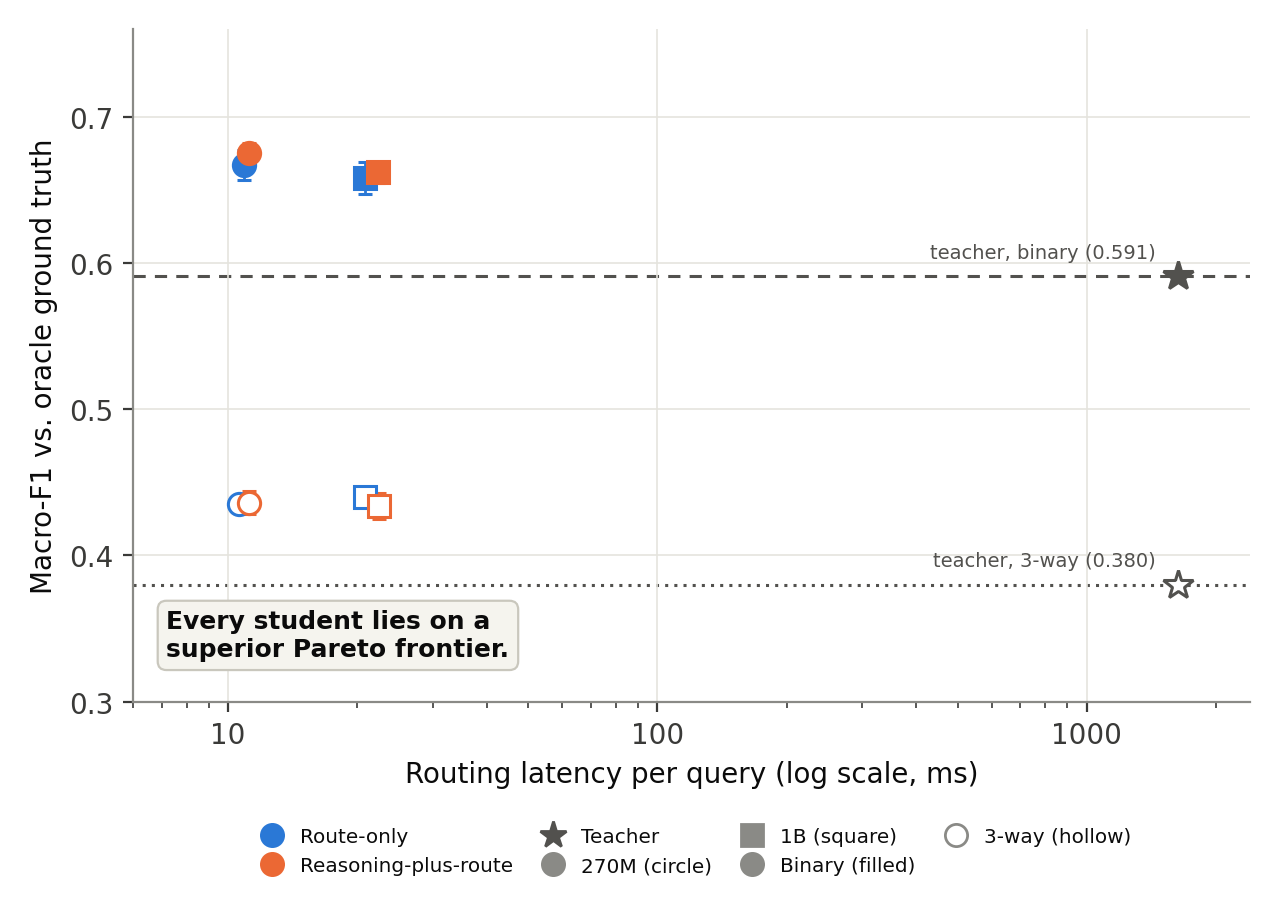
\includegraphics[width=0.6\linewidth]{figures/fig_pareto.png}
\end{figure}

Second, this advantage is not confined to the primary configuration.
Figure~\ref{fig:pareto} extends the comparison to all eight evaluated
distilled-router settings: every one achieves both lower latency and
higher oracle F1 than the teacher anchor for its own label space,
placing all eight on a strictly superior Pareto frontier.

Third, routing latency alone does not capture the full cost of serving a query: the routing decision's real purpose is to control the cost of \emph{answering} it, which also depends on the answer-generation latency of whichever candidate the decision selects. Figure~\ref{fig:cost-quality} places DistillRouter and the teacher against three fixed-policy baselines on this fuller cost (routing latency plus the expected answer-generation latency of the served candidate, weighted by the predicted-label distribution) versus end-to-end accuracy.

\begin{figure}[h]
\centering
\caption{\textbf{Cost-Quality Frontier} (binary label space, 270M
backbone). Expected cost per query in milliseconds of compute, log
scale (x-axis) vs.\ end-to-end accuracy (y-axis). Diamonds: fixed
policies that serve every query with one candidate. Star: the teacher.
Circles: DistillRouter, route-only (RO) and reasoning-plus-route (RR).
Dotted line: the oracle ceiling (0.542), the accuracy of always
picking the cheapest candidate that happens to answer correctly, an
upper bound no real policy can exceed. Cost is measured in compute
latency rather than dollar price (\ref{sec:datasets}).}
\label{fig:cost-quality}
\vspace{4pt}

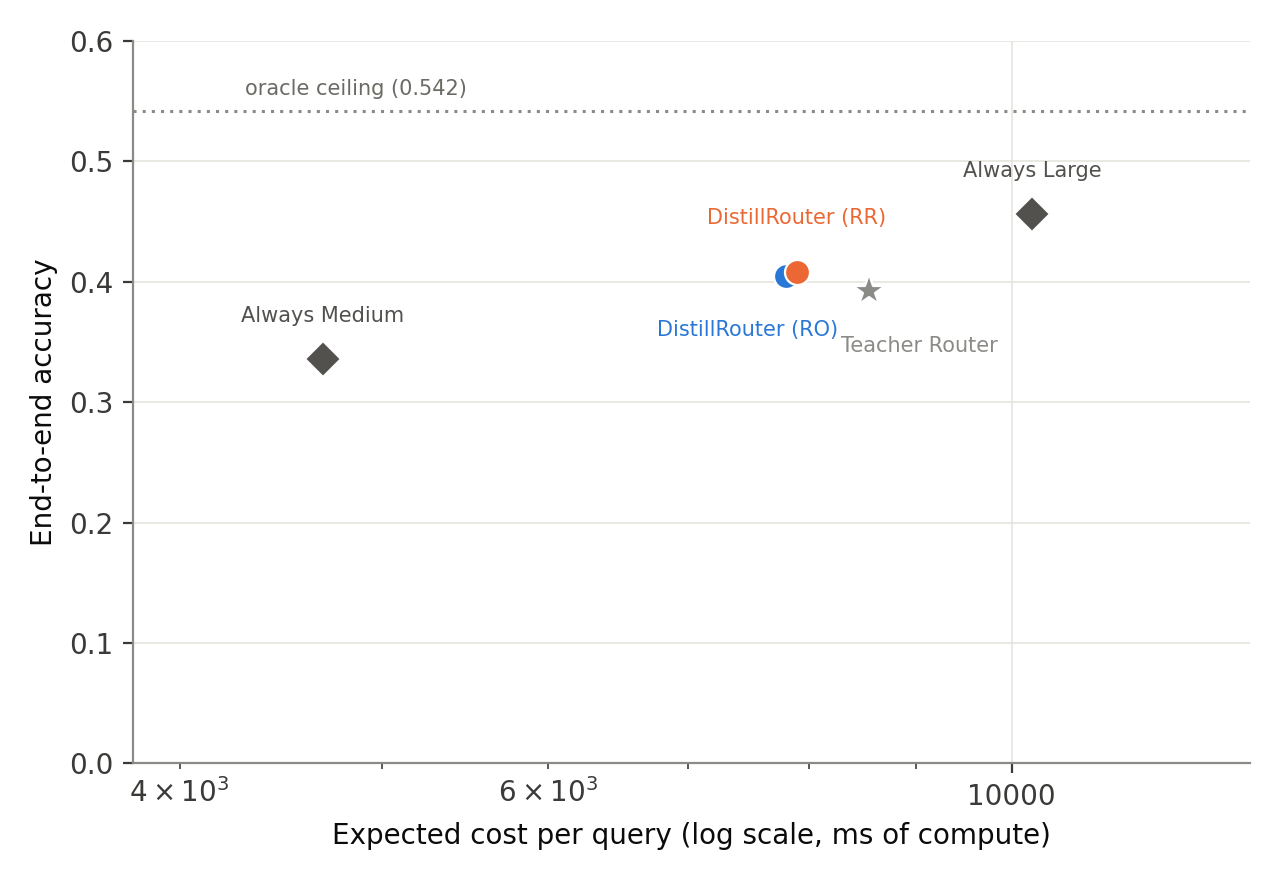
\includegraphics[width=0.55\linewidth]{figures/fig_cost_quality.png}
\end{figure}
On this view, the advantage narrows: both the teacher and DistillRouter fall between the Always-Medium and Always-Large baselines rather than beating either, and Always-Large retains the single highest raw accuracy of any point plotted. Routing therefore does not dominate the static Always-Large baseline in this aggregate view. Its value lies instead in the oracle-accuracy results above: routing identifies \emph{which} queries can safely stay on a cheaper candidate, a distinction the three-point plot cannot show. The gap to the oracle ceiling likewise shows substantial headroom remains for every policy plotted, including the teacher.

Together, these results show that routing policy transfers effectively into lightweight distilled models, delivering large, consistent oracle-accuracy and latency gains across every configuration tested — though end-to-end accuracy gains are smaller, and routing does not yet dominate the simplest static baseline.



\subsection{Deployment Efficiency}
\label{sec:rq3-efficiency}

\textbf{How much deployment efficiency can be gained through
distillation?}

Deployment efficiency is DistillRouter's primary motivation, and the
gains are large: shifting from the teacher's multi-stage prompting
process (\ref{sec:distillrouter_framework}) to a single forward pass
delivers speedups of up to 153× over the teacher, with routing
accuracy at or above the teacher's throughout
(\ref{sec:can-be-distilled}).

This holds across every evaluated configuration (Table~\ref{tab:mainperf}
for the primary configuration; Appendix Table~\ref{tab:efficiency}
for the remaining six): label-space granularity has little effect on
latency, and although scaling the backbone from 270M to 1B costs more,
substantial efficiency gains over the teacher remain.
\subsection{Reasoning Supervision and Policy Transfer}
\label{sec:main-result}
\textbf{RQ2: Does reasoning supervision improve policy transfer?}

Having established that distillation works and is efficient, we test
whether reasoning supervision improves it further. This section covers
policy transfer alone (agreement with the teacher's labels);
Section~\ref{sec:teacher-fidelity-oracle} covers whether the decisions
are actually correct. Two patterns emerge from Table~\ref{tab:main270m}.


\begin{table}[h]
\centering
\caption{\textbf{Policy Transfer Results.}
Macro-F1 against the teacher's decision, mean $\pm$ SD
across 10 seeds. $\Delta$ is route-only minus reasoning-plus-route on
macro-F1, with a 95\% CI from a paired bootstrap~\citep{koehn2004statistical} over the 10 seeds;
\textbf{bold} marks a CI that excludes zero.}
\label{tab:main270m}
\small
\begin{tabular}{@{}lrrr@{}}
\toprule
Configuration & RO F1 & RR F1 & $\Delta$ F1 (RO $-$ RR) \\
\midrule
Binary (270M)& 0.651 $\pm$ 0.005 & 0.645 $\pm$ 0.010 & $+0.0065$ ($[-0.0118, +0.0232]$) \\
Three-Label  & 0.477 $\pm$ 0.025 & 0.460 $\pm$ 0.018 & $+0.017$ ($[-0.022, +0.062]$) \\

\midrule

Binary (1B) & 0.652 $\pm$ 0.016 & 0.676 $\pm$ 0.008 & \textbf{$-0.024$ ($[-0.062, -0.003]$)} \\
Three-Label & 0.505 $\pm$ 0.012 & 0.529 $\pm$ 0.012 & \textbf{$-0.024$ ($[-0.055, -0.001]$)} \\
\bottomrule
\end{tabular}
\end{table}

First, scale matters: at the 270M backbone, route-only and
reasoning-plus-route distillation transfer the teacher's policy about
equally well, with confidence intervals overlapping on every metric
and including zero. At the larger 1B scale, however, reasoning
supervision produces a small but statistically reliable gain in policy
transfer, consistent across both label spaces. Because this comparison
holds data, architecture, and seeds fixed and varies only the training
objective, the association rests on firmer footing than a purely
observational correlation would, though it still comes from a single
teacher and task domain (\ref{sec:limitations}). This is consistent
with reasoning signals helping the router reproduce teacher behavior
more closely as capacity grows.

Second, and more surprisingly, this improved imitation does not
translate into better routing accuracy. At 1B, reasoning-plus-route
distillation's end-to-end accuracy is actually slightly \emph{lower}
than route-only's at both label spaces (\ref{sec:can-be-distilled}) —
the opposite direction from its confirmed fidelity advantage. A
single-configuration study would have reported just one of these
270M/1B outcomes as the general finding.

\subsection{Distilled Routers Achieve Higher Oracle Accuracy Than the Teacher}
\label{sec:distillation-improves-teacher}

A counterintuitive finding: distilled routers achieve higher oracle
accuracy than the teacher that supervised them
(Table~\ref{tab:mainperf}, \ref{sec:can-be-distilled}). Both are
measured against the same ground truth, so this is a direct
comparison, not an artifact of differing label distributions — yet the
distilled router is trained on nothing but the teacher's own labels.
We treat "the student exceeds the teacher" as a robust empirical
pattern, not a settled finding, and return to candidate explanations
below.

\begin{table}[h]
\centering
\caption{\textbf{Policy Transfer vs.\ Routing Accuracy}, mean $\pm$ SD
across 10 seeds, all four configurations, both metrics. In every row,
the oracle accuracy point estimate is at least as high as accuracy
against the teacher, though for Binary (1B) reasoning-plus-route the
two are within 0.002 of each other, well inside one SD (see prose
below); \textbf{bold} marks the higher-scoring variant in each F1
column, within each configuration, illustrating that accuracy and
macro-F1 do not always agree (e.g.\ Binary (1B) favors
reasoning-plus-route on accuracy but route-only on F1).}
\label{tab:teacher-oracle-accuracy}
\small
\begin{tabular}{@{}llrrrr@{}}
\toprule
Configuration & Variant & Acc vs.\ Teacher & Acc vs.\ Oracle & F1 vs.\ Teacher & F1 vs.\ Oracle \\
\midrule
\multirow{2}{*}{Binary (270M)} & Route-only & 0.652 $\pm$ 0.005 & 0.682 $\pm$ 0.011 & \textbf{0.651 $\pm$ 0.005} & 0.667 $\pm$ 0.010 \\
 & Reasoning-plus-route & 0.645 $\pm$ 0.011 & 0.692 $\pm$ 0.008 & 0.645 $\pm$ 0.010 & \textbf{0.675 $\pm$ 0.007} \\
\addlinespace
\multirow{2}{*}{Three-Label} & Route-only & 0.549 $\pm$ 0.010 & 0.636 $\pm$ 0.016 & \textbf{0.477 $\pm$ 0.025} & 0.435 $\pm$ 0.005 \\
 & Reasoning-plus-route & 0.545 $\pm$ 0.007 & 0.645 $\pm$ 0.015 & 0.460 $\pm$ 0.018 & \textbf{0.436 $\pm$ 0.008} \\
 \midrule
\addlinespace
\multirow{2}{*}{Binary (1B)} & Route-only & 0.652 $\pm$ 0.016 & 0.676 $\pm$ 0.014 & 0.652 $\pm$ 0.016 & 0.658 $\pm$ 0.011 \\
 & Reasoning-plus-route & 0.677 $\pm$ 0.008 & 0.679 $\pm$ 0.011 & \textbf{0.676 $\pm$ 0.008} & \textbf{0.662 $\pm$ 0.007} \\
 \addlinespace
\multirow{2}{*}{Three-Label} & Route-only & 0.574 $\pm$ 0.007 & 0.633 $\pm$ 0.010 & 0.505 $\pm$ 0.012 & \textbf{0.440 $\pm$ 0.007} \\
 & Reasoning-plus-route & 0.587 $\pm$ 0.014 & 0.629 $\pm$ 0.009 & \textbf{0.529 $\pm$ 0.012} & 0.434 $\pm$ 0.009 \\
\bottomrule
\end{tabular}
\end{table}

This pattern generalizes: Table~\ref{tab:teacher-oracle-accuracy} shows
the oracle-accuracy point estimate at or above teacher accuracy in all
eight configuration/variant pairs — though not uniformly: one cell
(Binary (1B), reasoning-plus-route) is close enough to call a tie, and
favors the teacher under macro-F1, consistent with
Section~\ref{sec:teacher-fidelity-oracle}'s broader finding that
accuracy and macro-F1 do not always agree. This pattern alone is
suggestive, not conclusive, since the teacher and oracle have
different label distributions; the controlled comparison above (same
ground truth for both) is what actually establishes the claim.

Nor is this simple memorization: the teacher systematically
under-predicts large-tier queries, and distilled routers substantially
recover these cases (Appendix~\ref{sec:error-analysis}) — learning a
more accurate escalation boundary than the teacher demonstrated,
rather than reproducing its errors.

Why would a classifier trained only on the teacher's own labels
outperform that teacher? The mechanism is not established; we see
three non-exclusive candidates: (1) \emph{regularization} — fitting
one boundary over many examples may average out per-query errors
rather than reproduce them; (2) \emph{prompting instability} — the
gap may reflect noise in the teacher's own two-stage prompting
(\ref{sec:teacher-policy}) rather than a general property of
distillation; (3) \emph{subtler contamination} — though splits are
disjoint and oracle labels are never used for training
(\ref{sec:oracle-routing-policy}), template overlap between GSM8K and
MATH cannot be fully ruled out. Distinguishing these, e.g.\ by
retraining against a deliberately degraded teacher, is left to future
work.

\subsection{Policy Transfer Does Not Predict Routing Accuracy}
\label{sec:teacher-fidelity-oracle}
\label{sec:fidelity-oracle-270m}

\textbf{RQ3: Do improvements in policy transfer translate into
improvements in routing accuracy?}

We compare each variant's policy transfer against its accuracy on
oracle labels, and find that imitating the teacher more closely does
not reliably mean being more correct.

\begin{figure}[h]
\centering
\caption{\textbf{Policy Transfer Does Not Predict Routing Accuracy.}
Teacher F1 (x-axis, fidelity) vs.\ oracle F1 (y-axis, correctness) for
route-only (RO) and reasoning-plus-route (RR) at all four
configurations (same marker convention as Figure~\ref{fig:pareto}),
the full rows of Table~\ref{tab:teacher-oracle-accuracy}. Dashed connectors join
same-configuration pairs; error bars are $\pm 1$ SD across 10 seeds.}
\label{fig:fidelity-vs-correctness}
\vspace{4pt}

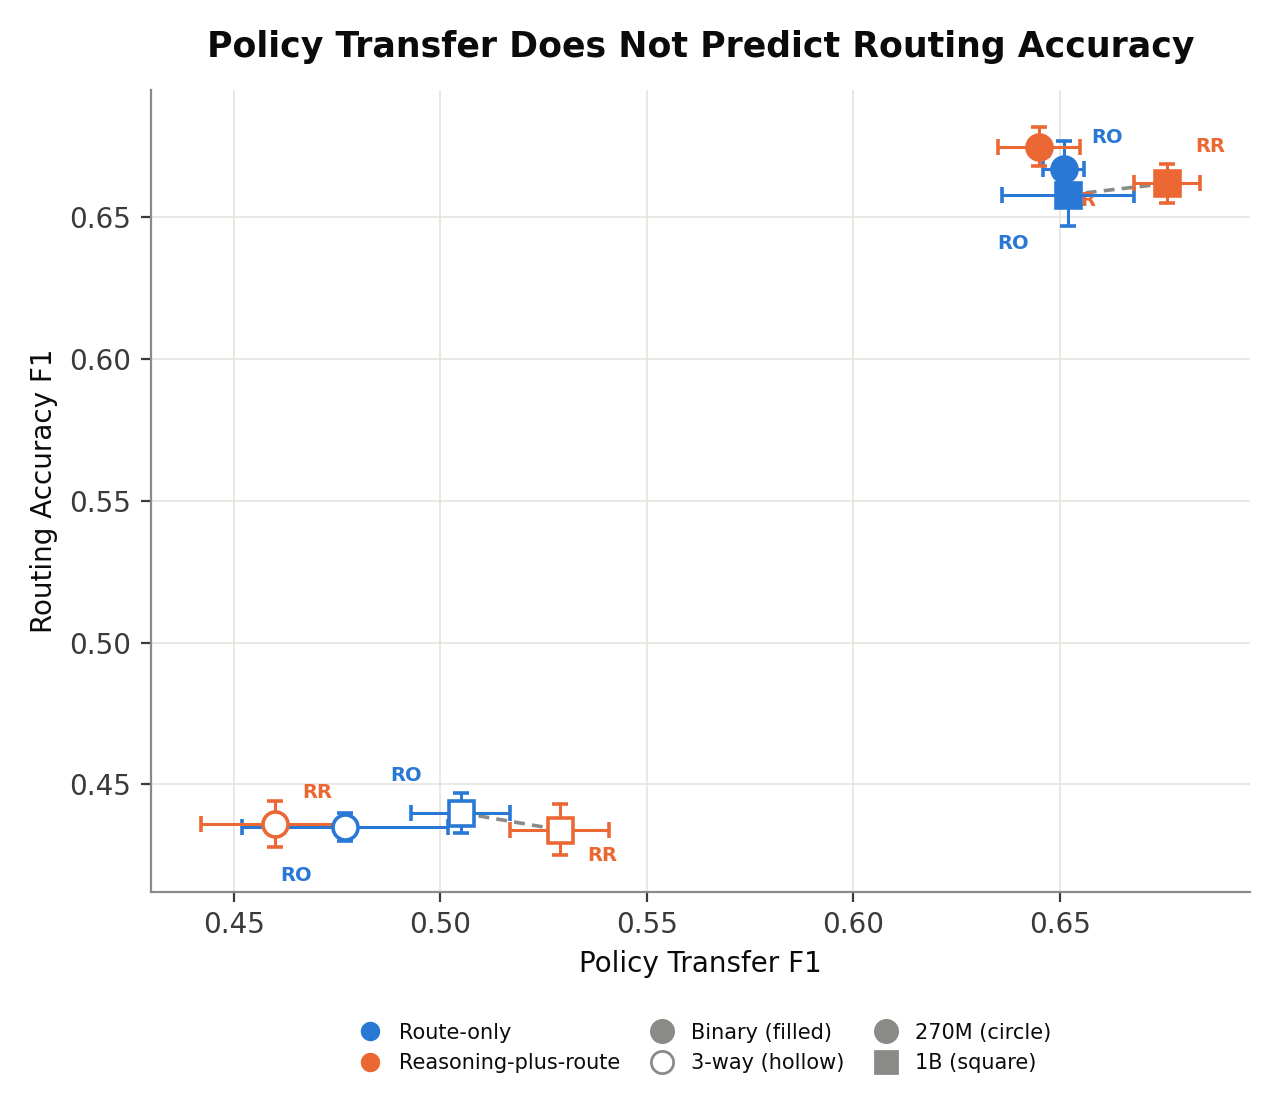
\includegraphics[width=0.6\linewidth]{figures/fig_fidelity_vs_correctness.png}
\end{figure}

Across configurations, the variant with higher teacher F1 does not
necessarily achieve higher oracle F1: at three of four configurations
the higher-teacher-F1 variant has \emph{lower} oracle-F1, and even
where rankings agree (binary/1B) the gap is not statistically
reliable. This holds even where the fidelity advantage itself is
confirmed (1B scale, \ref{sec:main-result}): no configuration shows a
statistically reliable oracle-F1 advantage for either variant.

To rule out a spurious correlation, not just an eight-point scatter: a
naive pooled correlation across all eight points is strongly positive
($r = +0.97$, $p < 0.001$), but this is a structural confound —
binary-label-space configurations score higher than three-label ones
on \emph{both} axes simply because binary is the easier problem
(Table~\ref{tab:teacher-oracle-accuracy}) — not evidence that fidelity
predicts correctness. Both a label-space-controlled partial
correlation (80 seed runs) and a direct paired test on the
reasoning-vs.-route-only \emph{change} (one point per configuration)
collapse this to null, confirming Figure~\ref{fig:fidelity-vs-correctness}'s
null correlation is not a sparse-scatter artifact; full statistics are
in Appendix~\ref{sec:correlation-appendix}.

Policy transfer and routing accuracy capture different aspects of
routing behavior and should not be treated as proxies for each other.
Two further checks confirm this without changing the picture: scaling
the distilled-router backbone from 270M to 1B produces no reliable
oracle-accuracy advantage in either label space, across the full
2$\times$2 label-space-by-backbone grid — a low-capacity prediction
problem for which lightweight models already suffice
(Appendix~\ref{sec:effect-of-scale}); and a confusion-matrix analysis
pooling all 10 seeds shows the accuracy gains reported above
concentrate in one failure mode — the teacher under-escalates
\texttt{large}-tier queries at essentially chance level, which
distillation corrects specifically rather than improving uniformly
(Appendix~\ref{sec:error-analysis}).

\section{Limitations}
\label{sec:limitations}

This study has several limitations. First, experiments are restricted to mathematical reasoning benchmarks; generalization to other domains (e.g., coding, open-domain QA) remains unverified. Second, we evaluate a single, non-frontier teacher (Qwen2.5-3B-Instruct, fixed two-stage prompt, not tuned for accuracy; \ref{sec:datasets}); whether a frontier-scale or more heavily prompt-engineered teacher would change the transfer characteristics we report, including the student-exceeds-teacher effect (Section~\ref{sec:distillation-improves-teacher}), is untested. Third, our scaling analysis covers only two backbone sizes, limiting conclusions across broader capacity ranges. Finally, reasoning is studied only as a training-time signal; its interaction with inference-time reasoning-based routing is not investigated.

\section{Conclusion}
\label{sec:conclusion}

We presented DistillRouter, a routing-policy distillation framework for efficient LLM routing. DistillRouter transfers routing policy from an expensive teacher router into a lightweight distilled model, enabling routing decisions through a single forward pass. Across multiple routing configurations, distilled routers achieved higher oracle-label accuracy than the teacher used to supervise them while reducing routing latency by up to 153×, though the mechanism behind this gap remains an open question (Section~\ref{sec:distillation-improves-teacher}). We further found that reasoning supervision is associated with improved policy transfer at larger scales but is not consistently associated with improved routing correctness. Overall, our results support the conclusion that routing policies can be effectively compressed through knowledge distillation, suggesting a practical approach for reducing routing overhead in large-scale LLM deployment.

\bibliographystyle{plainnat}
\bibliography{references}



\appendix
\section{Appendix}
\label{sec:appendix}

Section~\ref{sec:related-work} surveys prior work in full. Sections~\ref{sec:splits-appendix}--\ref{sec:error-analysis}
extend the main body's Experimental Setup and Results sections
(dataset splits, candidate models, teacher prompting details, training
hyperparameters, metric definitions, per-configuration efficiency,
scaling behavior, and error analysis) at the same 10-seed standard
used throughout the main body. The remaining checks below
(\ref{sec:loss-weighting} onward) are single-seed diagnostics, not
held to that standard; this is noted individually in each.

\subsection{Related Work}
\label{sec:related-work}

\paragraph{LLM Routing.} LLM routing aims to reduce inference cost by selecting the most appropriate model for each query. Recent work has shown that routing can significantly improve cost-quality tradeoffs compared to always using the most capable model. RouteLLM~\citep{ong2024routellm} learns lightweight routers from human preference data and dynamically selects between stronger and weaker models at inference time. ZOOTER~\citep{lu2024zooter} uses reward-model signals to train routing functions that dispatch queries to expert models. More recently, Router-R1\citep{zhang2025routerr1} formulates routing as a sequential decision-making problem and trains an LLM router through reinforcement learning, interleaving reasoning and routing actions.
While these approaches learn routing functions directly from preference labels, reward signals, or reinforcement learning, we instead distill the policy of an expensive teacher router into a lightweight deployable router — compressing an existing, costly policy rather than training a new one from preference, reward, or RL signals.

\paragraph{Routing Distillation and Reasoning Supervision.}

Knowledge distillation is widely used to transfer capabilities from large models to smaller ones, for example by using teacher-generated rationales as auxiliary training supervision~\citep{hsieh2023distilling}. Reasoning has also been explored as a mechanism for improving LLM decision making: in routing systems such as Router-R1, reasoning is generated during inference and contributes directly to routing decisions; closer to our setting, \citet{xu2025dualhead} train a classifier with an auxiliary reasoning head used only during training and dropped at inference, improving classifier accuracy without added inference cost. By contrast, we investigate reasoning as a training-time-only auxiliary supervisory signal specifically for routing-policy distillation, discarded at deployment, to study whether reasoning improves routing-policy transfer without increasing inference cost.

\subsection{Dataset Splits}
\label{sec:splits-appendix}

\begin{table}[h]
\centering
\caption{Split sizes and the oracle's routing-label distribution
(percentage of queries whose cheapest-correct tier is small/medium/
large), measured on the training split, independent of any teacher.}
\label{tab:splits}
\begin{tabular}{@{}lrrrrrr@{}}
\toprule
Dataset & Train & Validation & Test & Small & Medium & Large \\
\midrule
GSM8K & 1,000 & 747 & 500 & 6.8\% & 51.8\% & 41.4\% \\
MATH & 1,000 & 749 & 500 & 4.0\% & 24.6\% & 71.4\% \\
\textbf{Combined} & \textbf{2,000} & \textbf{1,496} & \textbf{1,000} & \textbf{5.4\%} & \textbf{38.2\%} & \textbf{56.4\%} \\
\bottomrule
\end{tabular}
\end{table}

\subsection{Candidate Models}
\label{sec:models-appendix}

\begin{table}[h]
\centering
\caption{Candidate answering models and the teacher router used to generate routing supervision.}
\label{tab:models}
\begin{tabular}{@{}llrp{6cm}@{}}
\toprule
Tier & Model & Parameters & Role \\
\midrule
Small & Gemma-3-270M & 268M & Cheapest candidate; also the distilled models' shared backbone \\
Medium & Qwen2.5-0.5B & 494M & Medium-cost candidate \\
Large & Gemma-3-1B & 1.0B & Most capable/expensive candidate \\
Teacher & Qwen2.5-3B-Instruct & 3.1B & Prompted only, never fine-tuned; reasoning zero-shot, route few-shot \\
\bottomrule
\end{tabular}
\end{table}

\subsection{Teacher Configuration Details}
\label{sec:teacher-config-appendix}
\label{sec:teacher-policy}

The teacher router follows a two-stage prompting procedure. For each
query, a zero-shot prompt first generates a teacher reasoning trace
describing the query's reasoning requirements, and a few-shot prompt
then predicts a routing decision conditioned on both the query and
the generated reasoning trace. Few-shot demonstrations are sampled
from the calibration split (\ref{sec:datasets}) and remain fixed
throughout training and evaluation. The teacher router is
Qwen2.5-3B-Instruct.

\subsection{Distilled Router Training}
\label{sec:training-protocol}

We train the two routing-policy distillation variants introduced in Sections~\ref{sec:route-only} and~\ref{sec:reasoning-plus-route} — route-only (teacher routing labels only) and reasoning-plus-route (additionally, teacher reasoning traces) — with all other training aspects identical, isolating the effect of reasoning supervision. Unless otherwise specified, all distilled routers are trained with the AdamW optimizer~\citep{loshchilov2019decoupled} at a learning rate of $2 \times 10^{-5}$, batch size 8, bf16 mixed precision, and 3 training epochs, selected using validation macro-F1 (imbalanced routing labels) and evaluated once on the held-out test split. Each main experiment is repeated across 10 seeds, with results reported as mean $\pm$ standard deviation.

\subsection{Evaluation Metric Definitions}
\label{sec:eval-metrics-appendix}

\paragraph{Policy Transfer.}
\label{sec:routing-policy-transfer}
Policy transfer measures how closely a distilled router reproduces the teacher router's routing policy. We report accuracy and macro-F1 between distilled routing labels and teacher routing labels. This metric answers RQ1 and RQ2.

\paragraph{Routing Accuracy.}
\label{sec:routing-correctness}
Routing accuracy measures agreement with oracle labels rather than the teacher router. Accuracy and macro-F1 are computed against oracle labels and provide an independent measure of routing quality. This metric answers RQ3 by evaluating whether improvements in policy transfer correspond to improvements in routing accuracy.

\paragraph{Deployment Efficiency.}
\label{sec:efficiency}
We report routing latency and speedup relative to the teacher router.
\emph{Routing latency} is the wall-clock time from an already-tokenized
query to a routing decision: a single forward pass for the distilled
router (\ref{sec:student-router}), or the sum of the teacher's two
generation calls (\ref{sec:teacher-policy}). It excludes tokenization,
detokenization, model loading, and the candidate's own
\emph{answer-generation} latency, added back only in the cost-quality
analysis (Figure~\ref{fig:cost-quality}). Latencies are measured at
batch size one on the same GPU (NVIDIA GB10), as the mean over the
test split for one run, not seed-averaged like accuracy
(\ref{sec:training-protocol}).

\subsection{Efficiency Across All Configurations}
\label{sec:efficiency-appendix}

\begin{table}[h]
\centering
\caption{\textbf{Efficiency, Generalization Checks.} Latency and
speedup vs.\ the teacher for the label-space/backbone variants beyond
the primary configuration, whose latency and speedup are already
reported in Table~\ref{tab:mainperf}
(\ref{sec:main-result}, \ref{sec:effect-of-scale}). Teacher
latency is measured directly (mean over the pooled 1,000-query
test split).}
\label{tab:efficiency}
\begin{tabular}{@{}llrr@{}}
\toprule
Configuration & Variant & Latency (ms) & Speedup \\
\midrule
\multirow{2}{*}{270M, Three-Label} & Route-only & 10.6 & 153× \\
 & Reasoning-plus-route & 11.2 & 145× \\
\midrule
\multirow{2}{*}{1B, Three-Label} & Route-only & 20.8 & 78× \\
 & Reasoning-plus-route & 22.4 & 72× \\
\addlinespace
\multirow{2}{*}{1B, Binary} & Route-only & 20.8 & 78× \\
 & Reasoning-plus-route & 22.3 & 73× \\
\bottomrule
\end{tabular}
\end{table}

This holds across every evaluated configuration (Tables~\ref{tab:mainperf}
and~\ref{tab:efficiency}): label-space granularity has little effect on
latency, and although scaling the backbone from 270M to 1B costs more,
substantial efficiency gains over the teacher remain.

\subsection{Scaling Analysis}
\label{sec:effect-of-scale}
\label{sec:fidelity-oracle-1b}
\label{sec:binary-ablation}
\label{sec:label-space-granularity}

We next examine whether routing policy changes when scaling the
distilled-router backbone from 270M to 1B, at both label spaces,
completing the full 2×2 grid (label space $\times$ backbone). For the
most part, it does not.

Increasing model size produces only modest, noise-level changes in
oracle-measured accuracy in either direction (Oracle F1 column,
Table~\ref{tab:teacher-oracle-accuracy}): at three-label, route-only and
reasoning-plus-route distillation essentially swap rank between 270M
and 1B, landing well within one standard deviation of each other
throughout; at binary, both variants drift slightly lower from 270M to
1B, a small dip rather than a genuine crossover. In neither label
space does increasing router size produce a reliable routing-accuracy
advantage.

Interestingly, model size matters for one thing: the association
between reasoning supervision and policy transfer grows more apparent
at 1B (Table~\ref{tab:main270m}), suggesting larger routers better
absorb extra supervisory signal even when that signal does not improve
routing correctness. Taken together, these results imply routing may
be a low-capacity prediction problem for which lightweight models already
suffice, with performance limited more by the quality of supervision
(\ref{sec:main-result}) than by model size — encouraging news for
deployment.

\subsection{Error Analysis}
\label{sec:error-analysis}

To understand routing policy better, we analyze confusion matrices
pooling every test prediction across all 10 seeds and both datasets
($n = 10{,}000$ per variant) under the binary-routing formulation,
against oracle labels. The pattern is consistent: distillation's gains
concentrate in one specific failure mode rather than spreading evenly
across all decisions.

\begin{figure}[h]
\centering
\caption{\textbf{Teacher vs.\ Distilled Router, Both Against Oracle Ground
Truth} (binary label space). Row-normalized recall; ``Distilled Router'' is
route-only, this paper's primary configuration. On \texttt{large}-tier
queries (bottom row), the teacher is close to a coin flip
(49.6\% correct), while the distilled router correctly escalates 68.6\%
of the time.}
\label{fig:confusion-teacher-vs-student}
\vspace{4pt}

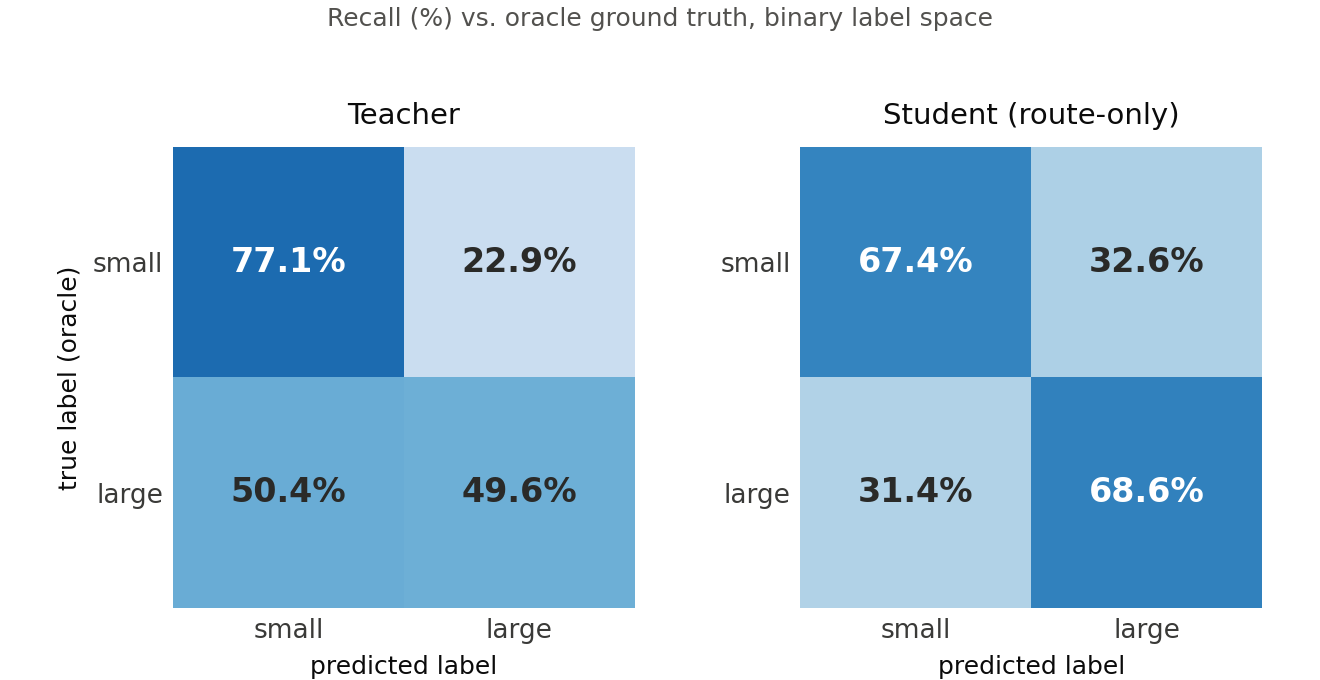
\includegraphics[width=0.65\linewidth]{figures/fig_confusion_teacher_vs_student.png}
\end{figure}

Against the oracle, the teacher itself under-escalates on large-tier
queries at essentially chance level
(Figure~\ref{fig:confusion-teacher-vs-student}). Both distilled
variants correct this specifically, recovering the large majority of
those large-tier queries at the cost of trading back a little
small-tier recall — this correction explains much of the accuracy
improvement reported in Section~\ref{sec:can-be-distilled}. Apart from
it, the two variants show highly similar error patterns. A smaller,
related asymmetry appears against the teacher's own decisions rather
than the oracle: a distilled model over-escalates roughly twice as
often as it under-escalates (42--44\% vs.\ 22--24\%), an ``err toward
the safer, more expensive tier'' bias that is separate from, and
smaller than, the oracle-referenced correction above. The remaining
errors largely reflect ambiguity near routing boundaries, where
queries could reasonably go either way.

These findings suggest distillation's primary benefit is not broad
improvement across all routing decisions, but correction of one
specific, important failure mode in the teacher.

\subsection{Correlation Test Details}
\label{sec:correlation-appendix}

We run three successively stricter correlation tests between
teacher-agreement F1 and oracle F1 to confirm the null relationship
reported in Section~\ref{sec:teacher-fidelity-oracle} is not an
artifact of the eight-point scatter. A naive Pearson correlation
across all eight points is strongly positive ($r = +0.97$,
$p < 0.001$), but this turns out to be a structural confound rather
than evidence that fidelity predicts correctness: binary-label-space
configurations score higher than three-label ones on \emph{both} axes
simply because binary is the easier problem
(Table~\ref{tab:teacher-oracle-accuracy}), inflating the pooled correlation without
reflecting any within-configuration relationship. Controlling for
label space removes it: a partial Pearson correlation over all 80
individual seed runs (10 seeds $\times$ 8 configuration/variant pairs)
residualized against a binary-vs.-three-label indicator collapses to
$r = -0.16$ ($p = 0.17$, $n = 80$). A more direct test confirms this,
correlating the reasoning-vs.-route-only \emph{change} in fidelity
against the corresponding change in oracle F1, one point per
configuration ($n = 4$): Pearson $r = -0.45$ ($p = 0.55$); Spearman
$\rho = 0.00$ ($p = 1.0$) — which configurations gain the most fidelity
carries no information about which gain the most accuracy. All three
tests agree once the label-space confound is removed.

\subsection{Loss Weight Sweep}
\label{sec:loss-weighting}

$\lambda_{\text{reason}} \in \{0.5, 1.0\}$ was swept at the 1B
backbone, three-label label space, single seed (42), best epoch per setting
(validation macro-F1): $\lambda_{\text{reason}} = 0.5$ reaches
$0.548$, $\lambda_{\text{reason}} = 1.0$ reaches $0.541$. $0.5$ was
selected and used throughout this paper's reasoning-plus-route runs.

\subsection{Seed Sensitivity}
\label{sec:seed-variance}

An initialization bug (the classification head was built before the
training seed was applied) produced a $0.060$ macro-F1 spread between
two nominally identical runs, roughly ten times the
route-only/reasoning-plus-route gap at the primary configuration
(Table~\ref{tab:main270m}). Fixed by seeding before model construction;
even after the fix, two seeds at the same setting still differed by
$0.023$: the motivation for the 10-seed protocol used throughout
this paper.

\subsection{Epoch-Count Robustness}
\label{sec:epoch-count}

Every main-body result uses a 3-epoch budget
(\ref{sec:training-protocol}). We checked this at a single seed (42),
20 epochs, both label spaces.

Both label spaces peak well past epoch 3 (binary: route-only at epoch
2, reasoning-plus-route at epoch 6; three-label: epoch 5 and 8
respectively), with validation macro-F1 gains of $0.08$--$0.12$ over
the 3-epoch checkpoint. On held-out test data, though, the gain is
smaller and inconsistent: route-only/binary (this paper's primary
configuration) is slightly \emph{worse} at its best 20-epoch
checkpoint (0.640) than the main protocol's 10-seed mean (0.651 $\pm$
0.005); the other three configurations indicate modest gains within
roughly one standard deviation.

Because route-only/binary is this paper's primary configuration, we
repeated it at 20 epochs across the same 10 seeds used throughout the
main protocol, rather than relying on the single-seed check above.
The 20-epoch test macro-F1 is $0.653 \pm 0.013$, against the 3-epoch
main-protocol result of $0.651 \pm 0.005$ (Table~\ref{tab:main270m}).
A paired seed-by-seed bootstrap over the 10 matched seeds gives a
mean improvement of $+0.002$ macro-F1 with a 95\% CI of
$[-0.006, +0.011]$, which includes zero: six of the 10 seeds are
lower at 20 epochs than at 3 epochs, and seed-to-seed variance nearly
triples ($\pm 0.013$ vs.\ $\pm 0.005$). Extending training therefore
does not yield a reliable test-set improvement at this configuration,
despite the consistent validation-macro-F1 gains observed above; this
confirms the single-seed result was not an artifact of that one seed,
and supports retaining the 3-epoch, 10-seed protocol as this paper's
main result.

\newpage
\section*{NeurIPS Paper Checklist}

\begin{enumerate}

\item {\bf Claims}
    \item[] Question: Do the main claims made in the abstract and introduction accurately reflect the paper's contributions and scope?
    \item[] Answer: \answerYes{}
    \item[] Justification: The abstract and Section~1's three contributions state exactly what is tested (route-only vs.\ reasoning-plus-route distillation, Section~3.3), the metrics used (transfer fidelity and macro-F1, Section~4.4), and the qualifying scope (two student backbones, one teacher configuration, two math datasets), matching the results in Section~5 and the limitations in Section~7.
    \item[] Guidelines:
    \begin{itemize}
        \item The answer \answerNA{} means that the abstract and introduction do not include the claims made in the paper.
        \item The abstract and/or introduction should clearly state the claims made, including the contributions made in the paper and important assumptions and limitations. A \answerNo{} or \answerNA{} answer to this question will not be perceived well by the reviewers. 
        \item The claims made should match theoretical and experimental results, and reflect how much the results can be expected to generalize to other settings. 
        \item It is fine to include aspirational goals as motivation as long as it is clear that these goals are not attained by the paper. 
    \end{itemize}

\item {\bf Limitations}
    \item[] Question: Does the paper discuss the limitations of the work performed by the authors?
    \item[] Answer: \answerYes{}
    \item[] Justification: Section~7 (Limitations) lists six specific limitations: only two student scales tested, single teacher configuration, limited robustness/multi-seed analysis (including the loss-weighting sweep not being re-run per seed or per scale), a fidelity-correctness reversal that is directionally consistent across seeds but not statistically reliable, domain specificity to mathematical reasoning, and the restricted scope of reasoning supervision studied.
    \item[] Guidelines:
    \begin{itemize}
        \item The answer \answerNA{} means that the paper has no limitation while the answer \answerNo{} means that the paper has limitations, but those are not discussed in the paper. 
        \item The authors are encouraged to create a separate ``Limitations'' section in their paper.
        \item The paper should point out any strong assumptions and how robust the results are to violations of these assumptions (e.g., independence assumptions, noiseless settings, model well-specification, asymptotic approximations only holding locally). The authors should reflect on how these assumptions might be violated in practice and what the implications would be.
        \item The authors should reflect on the scope of the claims made, e.g., if the approach was only tested on a few datasets or with a few runs. In general, empirical results often depend on implicit assumptions, which should be articulated.
        \item The authors should reflect on the factors that influence the performance of the approach. For example, a facial recognition algorithm may perform poorly when image resolution is low or images are taken in low lighting. Or a speech-to-text system might not be used reliably to provide closed captions for online lectures because it fails to handle technical jargon.
        \item The authors should discuss the computational efficiency of the proposed algorithms and how they scale with dataset size.
        \item If applicable, the authors should discuss possible limitations of their approach to address problems of privacy and fairness.
        \item While the authors might fear that complete honesty about limitations might be used by reviewers as grounds for rejection, a worse outcome might be that reviewers discover limitations that aren't acknowledged in the paper. The authors should use their best judgment and recognize that individual actions in favor of transparency play an important role in developing norms that preserve the integrity of the community. Reviewers will be specifically instructed to not penalize honesty concerning limitations.
    \end{itemize}

\item {\bf Theory assumptions and proofs}
    \item[] Question: For each theoretical result, does the paper provide the full set of assumptions and a complete (and correct) proof?
    \item[] Answer: \answerNA{}
    \item[] Justification: This is an empirical paper; it contains no theorems, lemmas, or formal proofs.
    \item[] Guidelines:
    \begin{itemize}
        \item The answer \answerNA{} means that the paper does not include theoretical results. 
        \item All the theorems, formulas, and proofs in the paper should be numbered and cross-referenced.
        \item All assumptions should be clearly stated or referenced in the statement of any theorems.
        \item The proofs can either appear in the main paper or the supplemental material, but if they appear in the supplemental material, the authors are encouraged to provide a short proof sketch to provide intuition. 
        \item Inversely, any informal proof provided in the core of the paper should be complemented by formal proofs provided in appendix or supplemental material.
        \item Theorems and Lemmas that the proof relies upon should be properly referenced. 
    \end{itemize}

    \item {\bf Experimental result reproducibility}
    \item[] Question: Does the paper fully disclose all the information needed to reproduce the main experimental results of the paper to the extent that it affects the main claims and/or conclusions of the paper (regardless of whether the code and data are provided or not)?
    \item[] Answer: \answerYes{}
    \item[] Justification: Section~3 describes the oracle/teacher/student pipeline in full, Section~4 specifies datasets, splits, models, and hyperparameters (learning rate, batch size, epochs, optimizer, precision, hardware), and Section~6 reports the loss-weighting sweep and the exact seeding fix applied to Variant~2, together sufficient to reconstruct every reported number.
    \item[] Guidelines:
    \begin{itemize}
        \item The answer \answerNA{} means that the paper does not include experiments.
        \item If the paper includes experiments, a \answerNo{} answer to this question will not be perceived well by the reviewers: Making the paper reproducible is important, regardless of whether the code and data are provided or not.
        \item If the contribution is a dataset and\slash or model, the authors should describe the steps taken to make their results reproducible or verifiable. 
        \item Depending on the contribution, reproducibility can be accomplished in various ways. For example, if the contribution is a novel architecture, describing the architecture fully might suffice, or if the contribution is a specific model and empirical evaluation, it may be necessary to either make it possible for others to replicate the model with the same dataset, or provide access to the model. In general. releasing code and data is often one good way to accomplish this, but reproducibility can also be provided via detailed instructions for how to replicate the results, access to a hosted model (e.g., in the case of a large language model), releasing of a model checkpoint, or other means that are appropriate to the research performed.
        \item While NeurIPS does not require releasing code, the conference does require all submissions to provide some reasonable avenue for reproducibility, which may depend on the nature of the contribution. For example
        \begin{enumerate}
            \item If the contribution is primarily a new algorithm, the paper should make it clear how to reproduce that algorithm.
            \item If the contribution is primarily a new model architecture, the paper should describe the architecture clearly and fully.
            \item If the contribution is a new model (e.g., a large language model), then there should either be a way to access this model for reproducing the results or a way to reproduce the model (e.g., with an open-source dataset or instructions for how to construct the dataset).
            \item We recognize that reproducibility may be tricky in some cases, in which case authors are welcome to describe the particular way they provide for reproducibility. In the case of closed-source models, it may be that access to the model is limited in some way (e.g., to registered users), but it should be possible for other researchers to have some path to reproducing or verifying the results.
        \end{enumerate}
    \end{itemize}


\item {\bf Open access to data and code}
    \item[] Question: Does the paper provide open access to the data and code, with sufficient instructions to faithfully reproduce the main experimental results, as described in supplemental material?
    \item[] Answer: \answerNo{}
    \item[] Justification: GSM8K and MATH (Section~4.1) are public benchmarks, but the oracle-labeling, teacher-prompting, and student-training code, together with the teacher-generated training data, are not yet released alongside this submission; Section~4 documents the procedure in enough detail to reimplement it in the interim.
    \item[] Guidelines:
    \begin{itemize}
        \item The answer \answerNA{} means that paper does not include experiments requiring code.
        \item Please see the NeurIPS code and data submission guidelines (\url{https://neurips.cc/public/guides/CodeSubmissionPolicy}) for more details.
        \item While we encourage the release of code and data, we understand that this might not be possible, so \answerNo{} is an acceptable answer. Papers cannot be rejected simply for not including code, unless this is central to the contribution (e.g., for a new open-source benchmark).
        \item The instructions should contain the exact command and environment needed to run to reproduce the results. See the NeurIPS code and data submission guidelines (\url{https://neurips.cc/public/guides/CodeSubmissionPolicy}) for more details.
        \item The authors should provide instructions on data access and preparation, including how to access the raw data, preprocessed data, intermediate data, and generated data, etc.
        \item The authors should provide scripts to reproduce all experimental results for the new proposed method and baselines. If only a subset of experiments are reproducible, they should state which ones are omitted from the script and why.
        \item At submission time, to preserve anonymity, the authors should release anonymized versions (if applicable).
        \item Providing as much information as possible in supplemental material (appended to the paper) is recommended, but including URLs to data and code is permitted.
    \end{itemize}


\item {\bf Experimental setting/details}
    \item[] Question: Does the paper specify all the training and test details (e.g., data splits, hyperparameters, how they were chosen, type of optimizer) necessary to understand the results?
    \item[] Answer: \answerYes{}
    \item[] Justification: Section~4.1 gives split sizes (Table~2) and answer-extraction rules; Section~4.3 gives the optimizer, learning rate, batch size, epoch count, precision, and hardware; Section~4.3--4.4 state that checkpoint selection used validation macro-F1 only, with the test split touched exactly once (Section~5.3).
    \item[] Guidelines:
    \begin{itemize}
        \item The answer \answerNA{} means that the paper does not include experiments.
        \item The experimental setting should be presented in the core of the paper to a level of detail that is necessary to appreciate the results and make sense of them.
        \item The full details can be provided either with the code, in appendix, or as supplemental material.
    \end{itemize}

\item {\bf Experiment statistical significance}
    \item[] Question: Does the paper report error bars suitably and correctly defined or other appropriate information about the statistical significance of the experiments?
    \item[] Answer: \answerYes{}
    \item[] Justification: Table~4 reports mean $\pm$ SD across ten independently seeded training runs per variant (Section~5.3), and the same ten seeds are used for a paired bootstrap (10,000 resamples) over both the teacher-fidelity comparison (Table~4) and the oracle-correctness comparison (Table~5), each reported with a 95\% CI and an explicit statement of whether that CI excludes zero. Section~5.5 repeats the identical ten-seed protocol at a second student backbone, again with paired-bootstrap CIs, and Section~5.6 repeats the oracle-correctness comparison at that same second backbone (Table~10), again with a paired-bootstrap CI. Section~6.2 additionally reports the two-seed parameter-initialization spread (0.023 macro-F1) that originally motivated moving to a multi-seed protocol. The source of variability (training seed, resampled via paired bootstrap) and the method (paired bootstrap over seeds, and separately over pooled test queries) are stated in Section~5.3; error bars in Tables~4--6 are sample standard deviations across seeds, not standard errors.
    \item[] Guidelines:
    \begin{itemize}
        \item The answer \answerNA{} means that the paper does not include experiments.
        \item The authors should answer \answerYes{} if the results are accompanied by error bars, confidence intervals, or statistical significance tests, at least for the experiments that support the main claims of the paper.
        \item The factors of variability that the error bars are capturing should be clearly stated (for example, train/test split, initialization, random drawing of some parameter, or overall run with given experimental conditions).
        \item The method for calculating the error bars should be explained (closed form formula, call to a library function, bootstrap, etc.)
        \item The assumptions made should be given (e.g., Normally distributed errors).
        \item It should be clear whether the error bar is the standard deviation or the standard error of the mean.
        \item It is OK to report 1-sigma error bars, but one should state it. The authors should preferably report a 2-sigma error bar than state that they have a 96\% CI, if the hypothesis of Normality of errors is not verified.
        \item For asymmetric distributions, the authors should be careful not to show in tables or figures symmetric error bars that would yield results that are out of range (e.g., negative error rates).
        \item If error bars are reported in tables or plots, the authors should explain in the text how they were calculated and reference the corresponding figures or tables in the text.
    \end{itemize}

\item {\bf Experiments compute resources}
    \item[] Question: For each experiment, does the paper provide sufficient information on the computer resources (type of compute workers, memory, time of execution) needed to reproduce the experiments?
    \item[] Answer: \answerYes{}
    \item[] Justification: Section~4.3 states both variants trained on a single NVIDIA GB10 GPU for 3 epochs at batch size 8 in bf16; Section~4.4 and Table~4 report per-query inference latency measured on the same GPU. We do not report a total-project compute estimate including preliminary or failed runs.
    \item[] Guidelines:
    \begin{itemize}
        \item The answer \answerNA{} means that the paper does not include experiments.
        \item The paper should indicate the type of compute workers CPU or GPU, internal cluster, or cloud provider, including relevant memory and storage.
        \item The paper should provide the amount of compute required for each of the individual experimental runs as well as estimate the total compute. 
        \item The paper should disclose whether the full research project required more compute than the experiments reported in the paper (e.g., preliminary or failed experiments that didn't make it into the paper). 
    \end{itemize}
    
\item {\bf Code of ethics}
    \item[] Question: Does the research conducted in the paper conform, in every respect, with the NeurIPS Code of Ethics \url{https://neurips.cc/public/EthicsGuidelines}?
    \item[] Answer: \answerYes{}
    \item[] Justification: The work uses only public math benchmarks (GSM8K, MATH) and openly available pretrained model checkpoints; it involves no human subjects, crowdsourcing, or personal data.
    \item[] Guidelines:
    \begin{itemize}
        \item The answer \answerNA{} means that the authors have not reviewed the NeurIPS Code of Ethics.
        \item If the authors answer \answerNo, they should explain the special circumstances that require a deviation from the Code of Ethics.
        \item The authors should make sure to preserve anonymity (e.g., if there is a special consideration due to laws or regulations in their jurisdiction).
    \end{itemize}


\item {\bf Broader impacts}
    \item[] Question: Does the paper discuss both potential positive societal impacts and negative societal impacts of the work performed?
    \item[] Answer: \answerNA{}
    \item[] Justification: This is foundational, methodological work on distilling routing policies for math question answering; it is not tied to a deployment and carries no direct path to a specific negative application beyond the general cost/quality trade-offs already inherent to any LLM-serving system, so a dedicated societal-impact discussion was not included.
    \item[] Guidelines:
    \begin{itemize}
        \item The answer \answerNA{} means that there is no societal impact of the work performed.
        \item If the authors answer \answerNA{} or \answerNo, they should explain why their work has no societal impact or why the paper does not address societal impact.
        \item Examples of negative societal impacts include potential malicious or unintended uses (e.g., disinformation, generating fake profiles, surveillance), fairness considerations (e.g., deployment of technologies that could make decisions that unfairly impact specific groups), privacy considerations, and security considerations.
        \item The conference expects that many papers will be foundational research and not tied to particular applications, let alone deployments. However, if there is a direct path to any negative applications, the authors should point it out. For example, it is legitimate to point out that an improvement in the quality of generative models could be used to generate Deepfakes for disinformation. On the other hand, it is not needed to point out that a generic algorithm for optimizing neural networks could enable people to train models that generate Deepfakes faster.
        \item The authors should consider possible harms that could arise when the technology is being used as intended and functioning correctly, harms that could arise when the technology is being used as intended but gives incorrect results, and harms following from (intentional or unintentional) misuse of the technology.
        \item If there are negative societal impacts, the authors could also discuss possible mitigation strategies (e.g., gated release of models, providing defenses in addition to attacks, mechanisms for monitoring misuse, mechanisms to monitor how a system learns from feedback over time, improving the efficiency and accessibility of ML).
    \end{itemize}
    
\item {\bf Safeguards}
    \item[] Question: Does the paper describe safeguards that have been put in place for responsible release of data or models that have a high risk for misuse (e.g., pre-trained language models, image generators, or scraped datasets)?
    \item[] Answer: \answerNA{}
    \item[] Justification: No models, datasets, or code are released with this submission; the trained routing classifiers pose no meaningful misuse risk beyond that of the publicly available base checkpoints they fine-tune.
    \item[] Guidelines:
    \begin{itemize}
        \item The answer \answerNA{} means that the paper poses no such risks.
        \item Released models that have a high risk for misuse or dual-use should be released with necessary safeguards to allow for controlled use of the model, for example by requiring that users adhere to usage guidelines or restrictions to access the model or implementing safety filters. 
        \item Datasets that have been scraped from the Internet could pose safety risks. The authors should describe how they avoided releasing unsafe images.
        \item We recognize that providing effective safeguards is challenging, and many papers do not require this, but we encourage authors to take this into account and make a best faith effort.
    \end{itemize}

\item {\bf Licenses for existing assets}
    \item[] Question: Are the creators or original owners of assets (e.g., code, data, models), used in the paper, properly credited and are the license and terms of use explicitly mentioned and properly respected?
    \item[] Answer: \answerNo{}
    \item[] Justification: Section~4.1--4.2 cites the origin of every dataset and model used (GSM8K \citep{cobbe2021training}, MATH \citep{hendrycks2021measuring}, Gemma-3, Qwen2.5), but the paper does not state each asset's license terms explicitly; we have not independently re-verified and reproduced those terms here.
    \item[] Guidelines:
    \begin{itemize}
        \item The answer \answerNA{} means that the paper does not use existing assets.
        \item The authors should cite the original paper that produced the code package or dataset.
        \item The authors should state which version of the asset is used and, if possible, include a URL.
        \item The name of the license (e.g., CC-BY 4.0) should be included for each asset.
        \item For scraped data from a particular source (e.g., website), the copyright and terms of service of that source should be provided.
        \item If assets are released, the license, copyright information, and terms of use in the package should be provided. For popular datasets, \url{paperswithcode.com/datasets} has curated licenses for some datasets. Their licensing guide can help determine the license of a dataset.
        \item For existing datasets that are re-packaged, both the original license and the license of the derived asset (if it has changed) should be provided.
        \item If this information is not available online, the authors are encouraged to reach out to the asset's creators.
    \end{itemize}

\item {\bf New assets}
    \item[] Question: Are new assets introduced in the paper well documented and is the documentation provided alongside the assets?
    \item[] Answer: \answerNA{}
    \item[] Justification: The paper does not release a new dataset, model, or code artifact alongside this submission; the teacher-generated training data and trained student checkpoints described in Sections~3--4 are not yet packaged for release.
    \item[] Guidelines:
    \begin{itemize}
        \item The answer \answerNA{} means that the paper does not release new assets.
        \item Researchers should communicate the details of the dataset\slash code\slash model as part of their submissions via structured templates. This includes details about training, license, limitations, etc. 
        \item The paper should discuss whether and how consent was obtained from people whose asset is used.
        \item At submission time, remember to anonymize your assets (if applicable). You can either create an anonymized URL or include an anonymized zip file.
    \end{itemize}

\item {\bf Crowdsourcing and research with human subjects}
    \item[] Question: For crowdsourcing experiments and research with human subjects, does the paper include the full text of instructions given to participants and screenshots, if applicable, as well as details about compensation (if any)?
    \item[] Answer: \answerNA{}
    \item[] Justification: The paper involves no crowdsourcing or human subjects; all data comes from existing math benchmarks and model-generated routing decisions.
    \item[] Guidelines:
    \begin{itemize}
        \item The answer \answerNA{} means that the paper does not involve crowdsourcing nor research with human subjects.
        \item Including this information in the supplemental material is fine, but if the main contribution of the paper involves human subjects, then as much detail as possible should be included in the main paper. 
        \item According to the NeurIPS Code of Ethics, workers involved in data collection, curation, or other labor should be paid at least the minimum wage in the country of the data collector. 
    \end{itemize}

\item {\bf Institutional review board (IRB) approvals or equivalent for research with human subjects}
    \item[] Question: Does the paper describe potential risks incurred by study participants, whether such risks were disclosed to the subjects, and whether Institutional Review Board (IRB) approvals (or an equivalent approval/review based on the requirements of your country or institution) were obtained?
    \item[] Answer: \answerNA{}
    \item[] Justification: The paper involves no human subjects research, so no IRB approval was sought or required.
    \item[] Guidelines:
    \begin{itemize}
        \item The answer \answerNA{} means that the paper does not involve crowdsourcing nor research with human subjects.
        \item Depending on the country in which research is conducted, IRB approval (or equivalent) may be required for any human subjects research. If you obtained IRB approval, you should clearly state this in the paper. 
        \item We recognize that the procedures for this may vary significantly between institutions and locations, and we expect authors to adhere to the NeurIPS Code of Ethics and the guidelines for their institution. 
        \item For initial submissions, do not include any information that would break anonymity (if applicable), such as the institution conducting the review.
    \end{itemize}

\item {\bf Declaration of LLM usage}
    \item[] Question: Does the paper describe the usage of LLMs if it is an important, original, or non-standard component of the core methods in this research? Note that if the LLM is used only for writing, editing, or formatting purposes and does \emph{not} impact the core methodology, scientific rigor, or originality of the research, declaration is not required.
    %this research?
    \item[] Answer: \answerYes{}
    \item[] Justification: LLMs are a core, original methodological component of this research, not just a writing aid: the teacher itself is a prompted LLM (Section~3.2) whose reasoning and routing decisions are the supervisory signal being distilled, and both student variants (Section~3.3) fine-tune a pretrained decoder-only LLM backbone.
    \item[] Guidelines:
    \begin{itemize}
        \item The answer \answerNA{} means that the core method development in this research does not involve LLMs as any important, original, or non-standard components.
        \item Please refer to our LLM policy in the NeurIPS handbook for what should or should not be described.
    \end{itemize}

\end{enumerate}

\end{document}
